\documentclass[11pt,a4paper]{article}

% Packages
\usepackage[utf8]{inputenc}
\usepackage[spanish, es-tabla]{babel}
\usepackage{amsmath}
\usepackage{amssymb}
\usepackage{upgreek}
\usepackage{accents}
\usepackage[shortlabels]{enumitem}
\usepackage{graphicx}
\usepackage{parskip}
\usepackage{array}
\usepackage[table]{xcolor}
\usepackage{tikz}		% Tener números dentro de cículos (\circled).
\usepackage{mdwlist} % Cambiar los índices en enumerate.
\usepackage{xfrac}		% Fracciones en diagonal (\sfrac).
\usepackage{lmodern} % Eliminar warning de Font shape.
\usepackage{mathtools}
\usepackage{xcolor}

% Definición de circled.
\newcommand*{\circled}[2][]{\tikz[baseline=(C.base)]{
	\node[inner sep=0pt] (C) {\vphantom{1g}#2};
	\node[draw, circle, inner sep=1pt, yshift=1pt]
		at (C.center) {\vphantom{1g}};}}
		
\newcolumntype{P}[1]{>{\centering\arraybackslash}p{#1}}
\newcolumntype{M}[1]{>{\centering\arraybackslash}m{#1}}
		
% Default fixed font does not support bold face
\DeclareFixedFont{\ttb}{T1}{txtt}{bx}{n}{12} % for bold
\DeclareFixedFont{\ttm}{T1}{txtt}{m}{n}{12}  % for normal

% Custom colors
\usepackage{color}
\definecolor{deepblue}{rgb}{0,0,0.5}
\definecolor{deepred}{rgb}{0.6,0,0}
\definecolor{deepgreen}{rgb}{0,0.5,0}

\usepackage{listings}

% Python style for highlighting
\newcommand\pythonstyle{\lstset{
language=Python,
basicstyle=\tiny,
morekeywords={self},              			% Add keywords here
keywordstyle=\color{deepblue},
emph={MyClass,__init__},          			% Custom highlighting
emphstyle=\ttb\color{deepred},    		% Custom highlighting style
stringstyle=\color{deepgreen},
frame=tb,                         					% Any extra options here
showstringspaces=false,
}}

% Python environment
\lstnewenvironment{python}[1][]
{
\pythonstyle
\lstset{#1}
}
{}

% Python for external files
\newcommand\pythonexternal[2][]{{
\pythonstyle
\lstinputlisting[#1]{#2}}}

% Python for inline
\newcommand\pythoninline[1]{{\pythonstyle\lstinline!#1!}}

\begin{document}
\begin{titlepage}
\centering

\includegraphics[width=0.15\textwidth]{./UGR.png}\par\vspace{1cm}
{\scshape\LARGE Universidad de Granada \par}
\vspace{1cm}
\vspace{1.5cm}
{\huge\bfseries Ingeniería del Conocimiento\par}
\vspace{2cm}
{\LARGE\bfseries Desarrollo de un sistema basado en el conocimiento\par}
\vspace{2cm}
{\Large\itshape Pedro Ramos Suárez\par}
\vspace{2cm}
{\Large\itshape DNI: 76591270M \par}
\vfill
Doble Grado de Ingeniería Informática y Matemáticas
\vfill
{\large \today\par}
\end{titlepage}

\tableofcontents

\newpage

\section{Selección de modelo}

En este sistema basado en el conocimiento tenemos dos funcionamientos:
\begin{enumerate}[label = \arabic*.]
\item Asesorar en que rama matricularse.
\item Dadas dos asignaturas, aconsejar cuál elegir.
\end{enumerate}

Por lo cuál, lo primero que hará al iniciarlo será preguntarnos que funcionamiento de los dos anteriores queremos que tenga.

A continuación explicamos en detalle como funciona cada uno.

\section{Asesorar en qué rama matricularse}

Las ramas posibles son las del grado en Ingeniería Informática: ``Computación y Sistemas Inteligentes'', ``Ingeniería del Software'', ``Ingeniería del Hardware'', ``Sistemas de Información'' y ``Tecnologías de la Información''.

La decisión de la rama en la que matricularse viene dada por el árbol:
\begin{center}
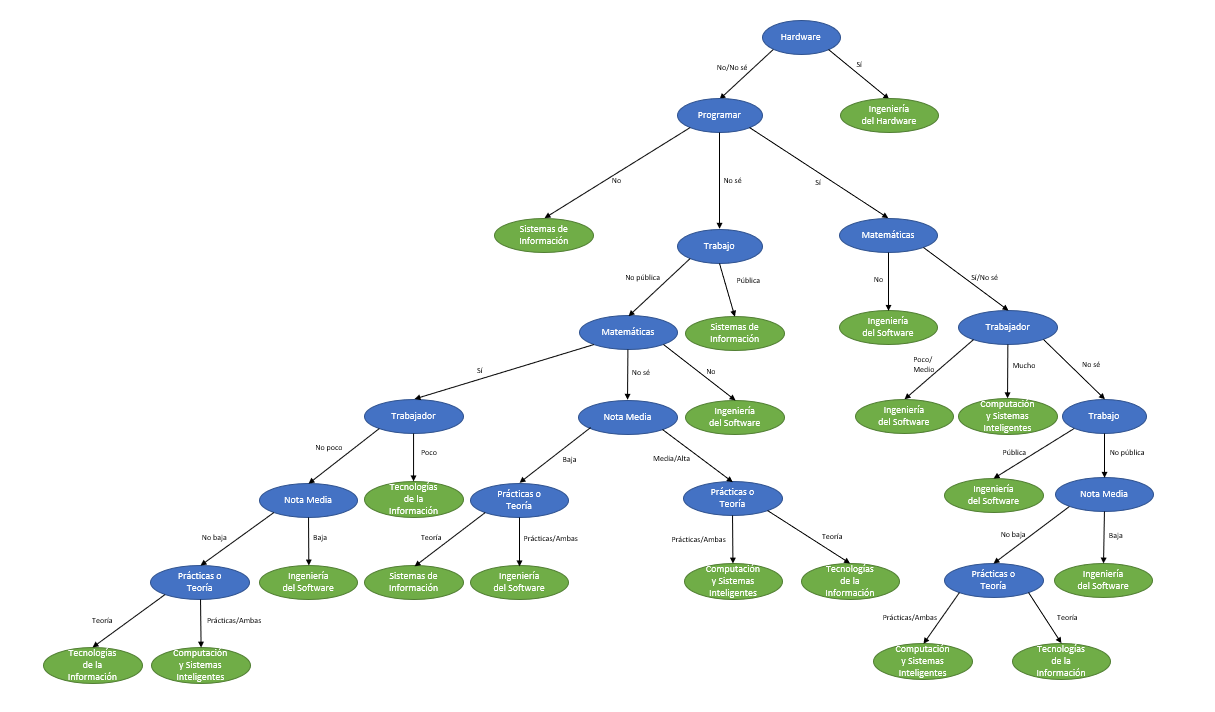
\includegraphics[scale=0.35]{./Tree.PNG}
\end{center}

(Incluyo la imagen ``Tree.PNG`` para poder ampliar el árbol de decisiones).

Por lo cuál, para decidir que rama recomendar, únicamente vamos recorriendo el árbol y en caso de que el nodo sea una pregunta, realizamos la pregunta, y en caso de que sea una recomendación, indicamos la rama y el motivo.

Además, en todas las entradas, comprobamos que la entrada sea válida, permitiendo varias opciones como ``Sí'', ``Si'', ``sí'' o ``si''.

Por lo cuál, en caso de que quisiéramos añadir una nueva pregunta que añadiese a alguna rama, tendríamos que modificar el nodo padre para añadir esta opción, y el nuevo nodo con la nueva rama.

Debido a que esta práctica pertenecía a la entrega anterior, no voy a entrar más en detalle.

\section{Aconsejar que asignatura elegir}

Para resolver este caso, usamos factores de certeza.

Para ello, primero preguntamos las dos asignaturas entre las que elegir. En mi caso, únicamente utilizo las cuatro asignaturas de la mención en ``Computación y Sistemas Inteligentes'' que he cursado: ``Ingeniería del Conocimiento'' (IC), ``Aprendizaje Automático'' (AA), ``Técnicas de los Sistemas Inteligentes' (TSI) y ``Modelos Avanzados de Computación'' (MAC), aunque es posible añadir más asignaturas.

Lo primero que realiza el sistema es pedir las dos asignaturas entre las que se duda, y comprueba que esta asignaturas son válidas. Ser válidas significan que son dos de las cuatro posibles explicadas previamente, y que sean distintas.

Una vez que tenemos las asignaturas, preguntamos por la información que necesitamos para hacer la recomendación, que es si le gustan las matemáticas, si le gusta programar, si prefiere las prácticas o la teoría y si prefiere asignaturas fáciles o difíciles. Todo esto lo preguntamos en una escala de 0 a 1, y comprobamos que la respuesta pertenezca a dicho intervalo. Usaremos este valor para poder aplicar factores de certeza, pero primero realizamos la siguiente transformación:

$$y = (x-1) * 2$$

donde $x$ era el valor introducido por el usuario. De esta manera, el valor que previamente estaba entre 0 y 1 ahora está entre -1 y 1, siendo 1 muy a favor, -1 muy en contra y 0 ni a favor ni en contra.

Luego utilizamos el procedimiento usado en la práctica 5 para obtener la certeza de cada valor, y finalmente elegimos el valor con mayor valor entre las asignaturas en las que dudaba el usuario.

Para justificar esta elección, debido a que hemos utilizado factores de certeza, nuestra única justificación es el valor de certeza obtenido para cada asignatura, el cuál imprimimos por pantalla.

Como he comentado previamente, podemos añadir más asignaturas. Para ello, lo único que tendríamos que realizar es:

\begin{enumerate}[label = \arabic*.]
\item Añadir la certeza inicial de esta asignatura, que debe ser 0. Para ello, si la asignatura es $Asignatura$, añadimos:
\begin{lstlisting}
(FactorCerteza Asignatura Si 0)
\end{lstlisting}
\item Añadir la asignatura a la lista de asignaturas que imprimimos por pantalla. Este paso no es necesario, pero facilita al usuario saber cuales son las asignaturas posibles.
\item Añadir el valor entre -1 y 1 que afecta cada una de las preguntas que realizamos. Es decir, si la asignatura $Asignatura$ que preguntamos será más recomendable para una persona a la que le guste las matemáticas en grado $x$, entonces añadiremos:
\begin{lstlisting}
(valor Asignatura Matematicas x)
\end{lstlisting}
\end{enumerate}

Con toda esta información, utilizando factores de certeza, puede calcular un valor entre -1 y 1 para cada asignatura, y nos devolverá el mayor de estos dos valores para las asignaturas que el usuario nos ha preguntado.

Además, en caso de que tuviésemos más asignaturas, también podríamos añadir más preguntas para poder una recomendación con más certeza. Para ello, si quisiéramos añadir la pregunta $Campo$, únicamente tendríamos que añadir:
\begin{lstlisting}
(valor Asignatura Campo x)
\end{lstlisting}
a todas las asignaturas del sistema.

\section{Conclusiones}

Debido a todo lo anterior, podemos concluir que el sistema es válido, ya que:

\begin{enumerate}[label = \arabic*]
\item Cubre las expectativas para las que fue construido, ya que asesora en qué rama matricularse y aconseja entre dos asignaturas, tal y como queríamos.
\item Explica sus respuestas. En el caso de asesorar la rama explica los motivos por lo cuál decide la rama recomendada, y en el caso de aconsejar entre dos asignaturas nos dice la certeza por la cual la ha elegido.
\item Permite añadir o modificar su conocimiento fácilmente, tal y como hemos explicado previamente.
\end{enumerate}

Las variables de entrada son todas las preguntas necesarias para el funcionamiento del sistema. Estas son si al usuario le gustan las matemáticas, si le gusta programar, si prefiere la teoría o las prácticas...

Las variables de salida son la rama o la asignatura recomendada, así como su justificación, dependiendo del funcionamiento solicitado por el usuario.

No utilizamos módulos, si no que tenemos todo el código junto. Podríamos dividir el programa en dos módulos, uno para cada funcionamiento del sistema, sin embargo es bastante simple, por lo que no es necesario.


\end{document}